%----------------------------------------------------------------------------
\chapter{\bevezetes}
%----------------------------------------------------------------------------

A IT technológiák térnyerésével egyre több és komplexebb rendszer készül, melyeknek sokszor valós időben kell működni. Mivel ilyen rendszerek jellemzően valamilyen biztonság kritikus környezetben működnek, elengedhetetlené válik ezek gondos megtervezése és átfogó vizsgálata különösen a helyes működés tekintetében.

A tervezés és ellenőrzés költséges, időigényes folyamat, ezért szükség van olyan eszközökre amelyek megkönnyítik vagy akár teljesen automatizálnak egyes folyamatokat. A tervezés során általában valamilyen modellvezért technikát alkalmaznak, melynek középpontjában a modellek állnak. Ennek lényege, hogy a tervezés során elkészített tervek nagyon sok értékes információt tartalmaznak, melyeket újra fel tudunk használni és származtatni ezekből kódot, dokumentációt, vagy akár más modelleket, ezáltal időt és erőforrásokat megtakarítva. Ráadásul mivel ezeket automatikusan gépek végzik, minimalizálódnak az emberi hibák például a programkódban, ahhoz képest mintha ezeket kézzel végeznénk el.

Terveinket már érdemes a tervezés korai fázisaiban ellenőrizni, hiszen az itt vétett hibák akár kritikusak lehetnek a későbbiekben. Az ellenőrzésekhez szintén fel tudjuk használni a modelljeinket és szimulálni tudjuk a rendszert, vagy képesek vagyunk a modellt közvetlen vizsgálni formális módszerek segítségével.

\begin{figure}[!ht]
	\centering
	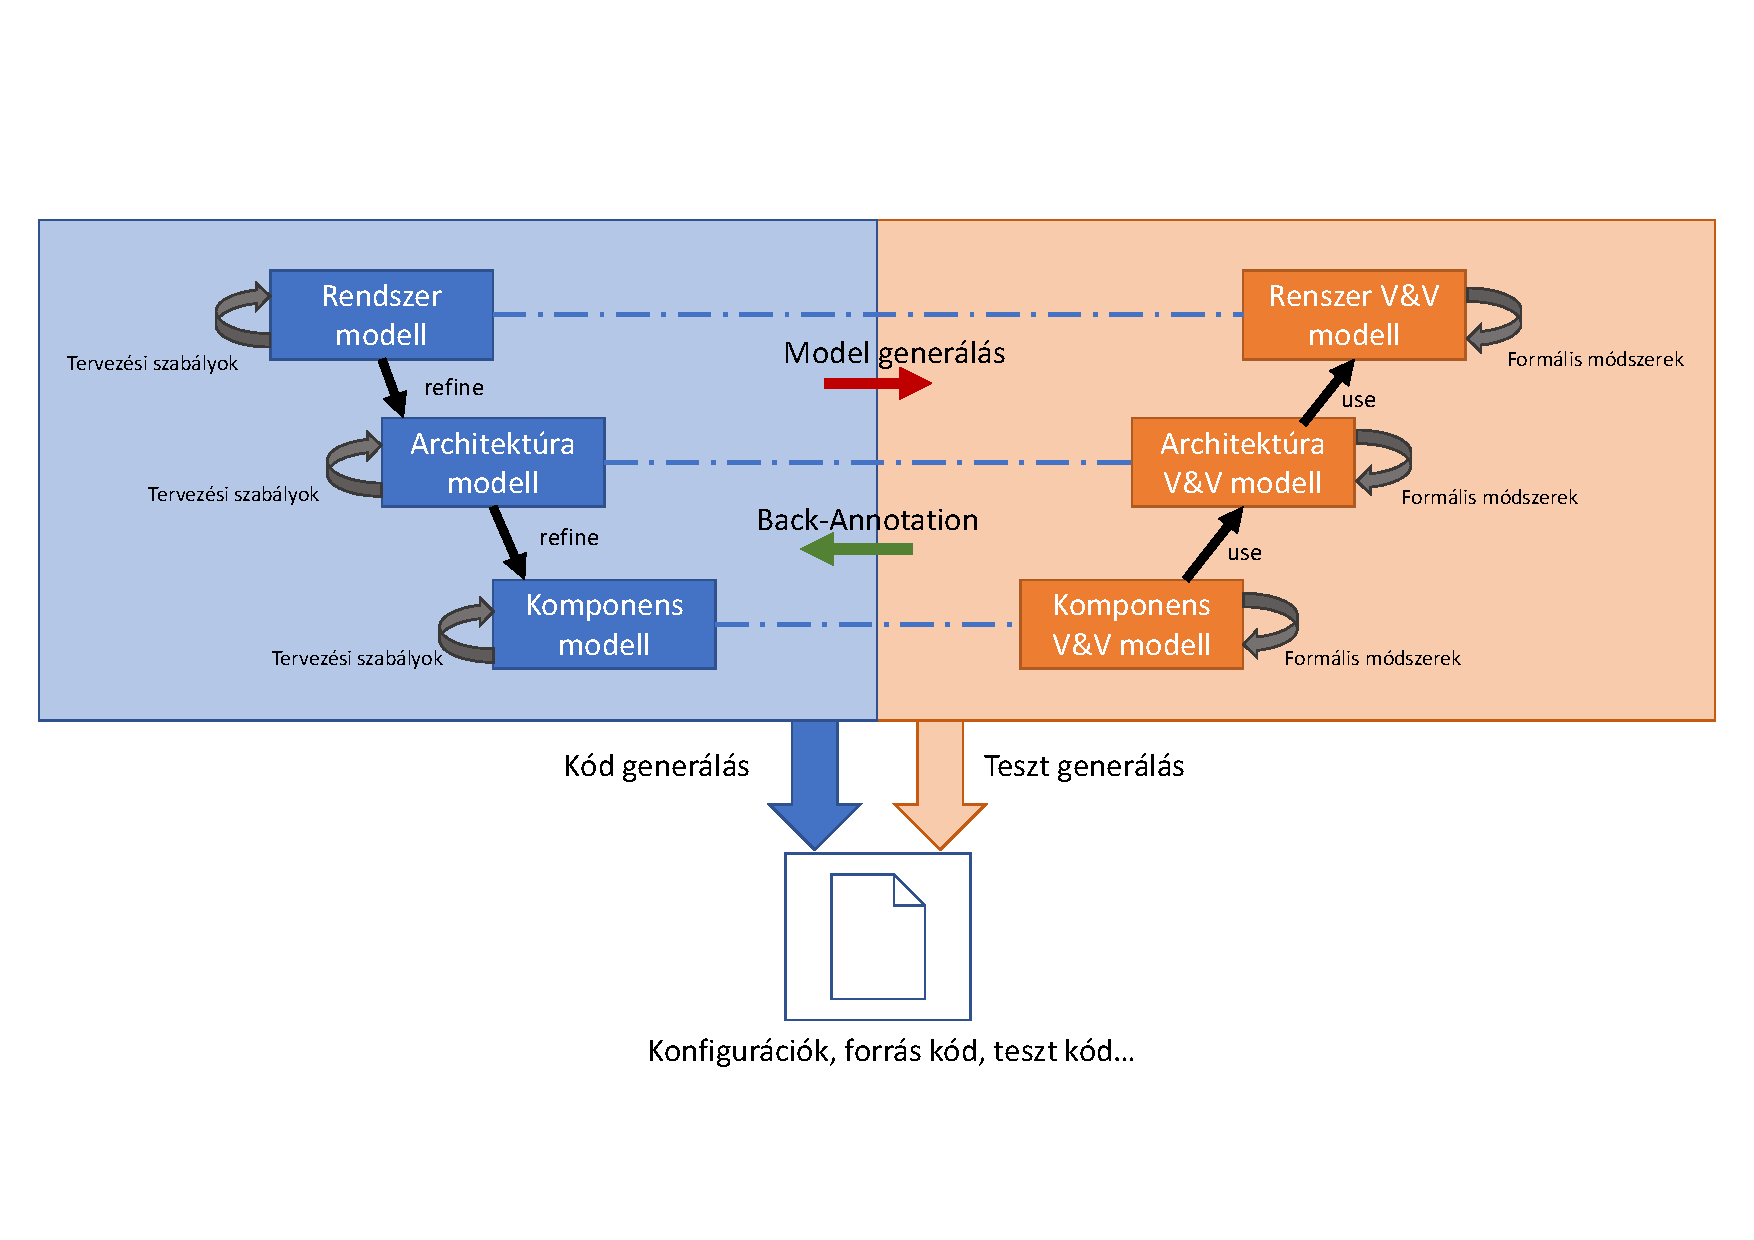
\includegraphics[width=120mm,keepaspectratio]{figures/Vmodel.pdf}
	\caption{Modell transzformációk kritikus rendszereknél}
	\label{fig:TeXstudio}
\end{figure}
